%!TeX root=../tese.tex
%("dica" para o editor de texto: este arquivo é parte de um documento maior)
% para saber mais: https://tex.stackexchange.com/q/78101/183146

%% ------------------------------------------------------------------------- %%
\chapter{Relação entre as delimitações de Wilber}
\label{cap:relacao-wilber}

Nesta capítulo estabeleceremos uma relação entre a delimitação da alternância e a delimitação do funil. Faremos isso por meio de um argumento geométrico a partir de uma caracterização nova de z-retângulos proposta por Lecomte e Weistein \cite{new_boundaries}.

%\section{Revisão histórica}

%Por muitos ano


\section{Novos conceitos}
Pouco se sabe sobre a relação entre a delimitação da alternância e do funil para sequências de acessos sem restrições. Assim, neste capítulo consideraremos apenas sequências de acessos sem repetições.

Seja $P$ um conjunto de pontos. Definimos a inversão temporal de um ponto $p \in P$ como $\widebar{p} = (p.x,-p.y)$. Definimos a inversão temporal de um conjunto de pontos $P$ como $\widebar{P} = \{\widebar{p} \mid p \in P\}$. Na prática, a inversão temporal de um conjunto de pontos é o conjunto resultante do espelhamento de cada um dos seus pontos em relação ao eixo das abscissas.

\begin{figure}
    \centering
    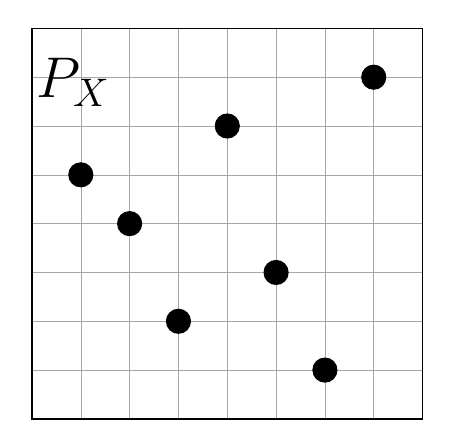
\begin{tikzpicture}[scale=0.62]
        \draw[very thin, gray!70] (0,0) grid (8,8);

        
        %\draw[red, line width=1.2pt] (1,5) rectangle (4,7);
        %\draw[red, line width=1.2pt] (3,3) rectangle (4,7);
        
        \filldraw[black] (6,1) circle (7pt);
        \filldraw[black] (3,2) circle (7pt);
        \filldraw[black] (5,3) circle (7pt);
        \filldraw[black] (2,4) circle (7pt);
        \filldraw[black] (1,5) circle (7pt);
        \filldraw[black] (4,6) circle (7pt);
        \filldraw[black] (7,7) circle (7pt);
        \draw[black, line width=0.5pt] (0,0) rectangle (8,8);

        \node[anchor=south west] at (-0.1,6.2) {\huge$P_X$};
    \end{tikzpicture}
    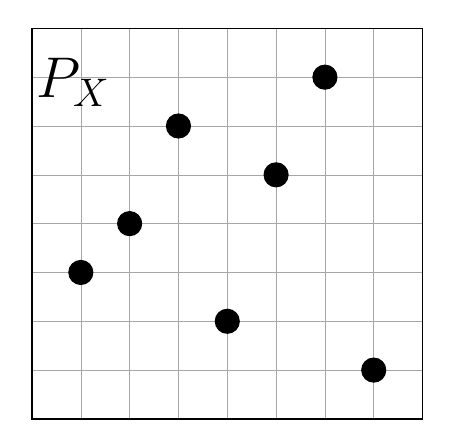
\begin{tikzpicture}[scale=0.62]
        \draw[very thin, gray!70] (0,0) grid (8,8);
        
        %\draw[black, line width=1.2pt] (5,2) rectangle (4,7);
        %\draw[black, line width=1.2pt] (6,6) rectangle (4,7);
        
        \filldraw[black] (7,1) circle (7pt);
        \filldraw[black] (4,2) circle (7pt);
        \filldraw[black] (1,3) circle (7pt);
        \filldraw[black] (2,4) circle (7pt);
        \filldraw[black] (5,5) circle (7pt);
        \filldraw[black] (3,6) circle (7pt);
        \filldraw[black] (6,7) circle (7pt);
        \draw[black, line width=0.5pt] (0,0) rectangle (8,8);

        \node[anchor=south west] at (-0.1,6.2) {\huge$\widebar{P_X}$};
    \end{tikzpicture}
    \caption{À esquerda, o conjunto de pontos $P_X$ relativo a sequência de acessos $X =(6,3,5,4,2,1,7) $. À direita, a inversão temporal de $P_X$.}
\end{figure}

\section{Relacionando a alternância com o funil e sua inversão temporal}

Primeiramente, é necessário entender como a inversão temporal de um ponto influencia a sua delimitação do funil.

\begin{comment}
\begin{lemma}
    Seja $p$ um ponto de um conjunto $P$. Se $p \in P_E$ então $f(P,p) \geq f(P_E,p)$ e $f(\widebar{P},\widebar{p}) \geq f(\widebar{P_E},\widebar{p})$. Se $p \in P_D$ então $f(P,p) \geq f(P_D,p)$ e $f(\widebar{P},\widebar{p}) \geq f(\widebar{P_D},\widebar{p})$.
\end{lemma}

\begin{proof}
    Suponha que $p \in P_E$. Como $p$ pertence a $P_E$ 
    Perceba que todos os pontos do funil esquerdo de $p$  
    
    Todos os pontos à esquerda de $p$ também pertencem a $P_E$, ou seja, $F_E(P_E,p) = F_E(P,p)$.
\end{proof}
\end{comment}

\begin{lemma} \label{lemma-relacao-alt-com-funil}
    Seja $P_X$ a visão geométrica de uma sequência de acessos sem repetições e $\cT$ uma árvore de referência em relação à $P_X$. Funil$(P_X) + $ Funil$(\widebar{P_X}) \geq $ Alt$_{\cT}(P_X)$.
\end{lemma}

\begin{proof}
    Faremos uma prova por indução em $k$ que, toda árvore $\cT$ de $k$ nós satisfaz a inequação do Lema.

    Para $k = 1$, a árvore de referência $\cT$ possui um único nó. Assim, Alt$_{\cT}(P_X) = 0$ e a inequação é valida.

    Suponha agora que $k > 1$ e que a propriedade vale para toda árvore com menos que $k$ nós. Seja $\cT_{L}$ e $\cT_{R}$ respectivamente a subárvore esquerda e a subárvore direita da raiz de $\cT$. Seja $P_L = \{p \in P_X \mid p.x \in \cT_L\}$ e $P_R = \{p \in P_X \mid p.x \in \cT_R\}$. Pela hipótese de indução, temos
    \begin{center}
    $\text{Funil}(P_E) +  \text{Funil}(\widebar{P_E}) \geq  \text{Alt}_{\cT_E}(P_E)$,

    $\text{Funil}(P_D) +  \text{Funil}(\widebar{P_D}) \geq  \text{Alt}_{\cT_D}(P_D)$.
    \end{center}
    Assim, sabemos que 
    \begin{align}
        \text{Alt}_{\cT}(P_X) &= a(P_X,\cT) + \text{Alt}_{\cT_E}(P_X) + \text{Alt}_{\cT_D}(P_X), \notag \\
        &\leq a(P_X,\cT) + \text{Funil}(P_E) +  \text{Funil}(\widebar{P_E}) + \text{Funil}(P_D) +  \text{Funil}(\widebar{P_D}). \label{eq:inicio}
    \end{align}

    Agora, é necessário entender como a delimitação do funil é afetada pela inversão temporal.
    Seja $p$ um ponto de $P_X$. Mostraremos que se $p \in P_E$, então $f(P_X,p) \geq f(P_E,p)$ e $f(\widebar{P_X},\widebar{p}) \geq f(\widebar{P_E},\widebar{p})$. De maneira simétrica, se $p \in P_D$ então $f(P_X,p) \geq f(P_D,p)$ e $f(\widebar{P_X},\widebar{p}) \geq f(\widebar{P_D},\widebar{p})$.

    Suponha que $p \in P_E$. Como $p$ pertence à $P_E$, então todos os pontos à esquerda de $p$ também pertencem à $P_E$, ou seja, $F_E(P_E,p) = F_E(P_X,p)$. Além disso, todos os pontos que pertencem à $P_E$ e estão à direita de $p$ pertencem a tanto o funil direito de $p$ em relação à $P_E$ quanto em relação à $P_X$, ou seja, $F_D(P_E,p) \subseteq F_D(P_X,p)$. Veja a Figura~\ref{fig:funis}. Assim, $mix(F_E(P_E,p).y,F_D(P_E,p).y)$ é uma subsequência de $mix(F_E(P_X,p).y,F_D(P_X,p).y)$, logo 

    \begin{center}
        $blocos(mix(F_E(P_E,p), F_D(P_E,p))) \leq blocos(mix(F_E(P_X,p), F_D(P_X,p)))$,

        $f(P_E,p) \leq f(P_X,p)$.
    \end{center}
    O argumento simetricamente vale para os outros casos.
    \begin{comment}
    \begin{figure}
        \centering
        \begin{minipage}[t]{0.3\textwidth}
        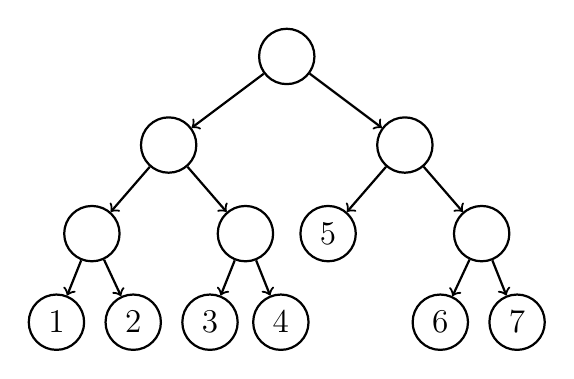
\begin{tikzpicture}[scale=0.75,
            node/.style={circle,draw,minimum size=2em, thick, font=\large},
            nodeGray/.style={circle,draw,minimum size=2em, thick, font=\large, fill=gray!55}]
            
            %\node[node] (D) at (0,0) {};
            %\node[node] (B) at (-1.5,-1.5) {};
            %\node[node] (A) at (-2.3,-3) {$1$};
            %\node[node] (C) at (-0.8,-3) {$2$};
            %\node[node] (E) at (0.8,-3) {$3$};
            %\node[node] (F) at (1.5,-1.5) {};
            %\node[node] (G) at (2.3,-3) {};
            %\node[node] (H) at (1.8,-4.5) {$4$};
            %\node[node] (I) at (2.9,-4.5) {$5$};
            
            \node[node] (D) at (0,0) {};
            \node[node] (B) at (-2,-1.5) {};
            \node[node] (A) at (-3.3,-3) {};
            \node[node] (C) at (-0.7,-3) {};
            \node[node] (E) at (0.7,-3) {$5$};
            \node[node] (F) at (2,-1.5) {};
            \node[node] (G) at (3.3,-3) {};
            \node[node] (H) at (2.6,-4.5) {$6$};
            \node[node] (I) at (3.9,-4.5) {$7$};
            \node[node] (J) at (-3.9,-4.5) {$1$};
            \node[node] (K) at (-2.6,-4.5) {$2$};
            \node[node] (L) at (-1.3,-4.5) {$3$};
            \node[node] (M) at (-0.1,-4.5) {$4$};
            
            \draw[thick, ->] (D) -- (B);%node[midway, left, yshift=0.15cm, xshift=0.08cm] {\textbf{E}};
            \draw[thick, ->] (B) -- (A);%node[midway, left, yshift=0.15cm, xshift=0.08cm] {\textbf{E}};
            \draw[thick, ->] (B) -- (C);%node[midway, right, yshift=0.15cm, xshift=-0.08cm] {\textbf{D}};
            \draw[thick, ->] (G) -- (I);%node[midway, right, yshift=0.15cm, xshift=-0.08cm] {\textbf{D}};
            \draw[thick, ->] (G) -- (H);%node[midway, left, yshift=0.15cm, xshift=0.08cm] {\textbf{E}};
            \draw[thick, ->] (A) -- (J);%node[midway, left, yshift=0.15cm, xshift=0.08cm] {\textbf{E}};
            \draw[thick, ->] (A) -- (K);%node[midway, left, yshift=0.15cm, xshift=0.08cm] {\textbf{E}};
            \draw[thick, ->] (C) -- (L);%node[midway, left, yshift=0.15cm, xshift=0.08cm] {\textbf{E}};
            \draw[thick, ->] (C) -- (M);%node[midway, left, yshift=0.15cm, xshift=0.08cm] {\textbf{E}};
            
            \draw[thick, ->] (D) -- (F);%node[midway, right, yshift=0.15cm, xshift=-0.08cm] {\textbf{D}};
            \draw[thick, ->] (F) -- (E);%node[midway, left, yshift=0.15cm, xshift=0.08cm] {\textbf{E}};
            \draw[thick, ->] (F) -- (G);%node[midway, right, yshift=0.15cm, xshift=-0.08cm] {\textbf{D}};
        
        \end{tikzpicture}
        \end{minipage}
        \hfill    
        \begin{minipage}[t]{0.7\textwidth}
        \begin{tikzpicture}[scale=0.45]
            \draw[very thin, gray!70] (0,0) grid (8,8);
            \draw[fill=gray!90, gray!90] (8,0) rectangle (4.5,8);
    
            \draw[color_of_analysed_point, dashed, line width=1.5pt] (3,0) -- (3,8);
            
            %\draw[red, line width=1.2pt] (1,5) rectangle (4,7);
            %\draw[red, line width=1.2pt] (3,3) rectangle (4,7);
            
            \filldraw[black] (4,1) circle (7pt);
            \filldraw[black] (6,2) circle (7pt);
            \filldraw[red] (2,3) circle (7pt);
            \filldraw[black] (5,4) circle (7pt);
            \filldraw[red] (1,5) circle (7pt);
            \filldraw[black] (7,6) circle (7pt);
            \filldraw[color_of_analysed_point] (3,7) circle (7pt);
            \draw[black, line width=0.5pt] (0,0) rectangle (8,8);
        \end{tikzpicture}
        \begin{tikzpicture}[scale=0.45]
            \draw[very thin, gray!70] (0,0) grid (8,8);
            \draw[fill=gray!90, gray!90] (8,0) rectangle (4.5,8);
    
            \draw[color_of_analysed_point, dashed, line width=1.5pt] (3,0) -- (3,8);
            
            %\draw[red, line width=1.2pt] (1,5) rectangle (4,7);
            %\draw[red, line width=1.2pt] (3,3) rectangle (4,7);
            
            \filldraw[red] (4,1) circle (7pt);
            \filldraw[black] (6,2) circle (7pt);
            \filldraw[black] (2,3) circle (7pt);
            \filldraw[black] (5,4) circle (7pt);
            \filldraw[black] (1,5) circle (7pt);
            \filldraw[black] (7,6) circle (7pt);
            \filldraw[color_of_analysed_point] (3,7) circle (7pt);
            \draw[black, line width=0.5pt] (0,0) rectangle (8,8);
        \end{tikzpicture}  
        \\
        \begin{tikzpicture}[scale=0.45]
            \draw[very thin, gray!70] (0,0) grid (8,8);
    
            \draw[color_of_analysed_point, dashed, line width=1.5pt] (3,0) -- (3,8);
            
            %\draw[red, line width=1.2pt] (1,5) rectangle (4,7);
            %\draw[red, line width=1.2pt] (3,3) rectangle (4,7);
            
            \filldraw[black] (4,1) circle (7pt);
            \filldraw[black] (6,2) circle (7pt);
            \filldraw[red] (2,3) circle (7pt);
            \filldraw[black] (5,4) circle (7pt);
            \filldraw[red] (1,5) circle (7pt);
            \filldraw[black] (7,6) circle (7pt);
            \filldraw[color_of_analysed_point] (3,7) circle (7pt);
            \draw[black, line width=0.5pt] (0,0) rectangle (8,8);
        \end{tikzpicture}
        \begin{tikzpicture}[scale=0.45]
            \draw[very thin, gray!70] (0,0) grid (8,8);
    
            \draw[color_of_analysed_point, dashed, line width=1.5pt] (3,0) -- (3,8);
            
            %\draw[red, line width=1.2pt] (1,5) rectangle (4,7);
            %\draw[red, line width=1.2pt] (3,3) rectangle (4,7);
            
            \filldraw[red] (4,1) circle (7pt);
            \filldraw[black] (6,2) circle (7pt);
            \filldraw[black] (2,3) circle (7pt);
            \filldraw[red] (5,4) circle (7pt);
            \filldraw[black] (1,5) circle (7pt);
            \filldraw[red] (7,6) circle (7pt);
            \filldraw[color_of_analysed_point] (3,7) circle (7pt);
            \draw[black, line width=0.5pt] (0,0) rectangle (8,8);
        \end{tikzpicture} 
        \end{minipage}
        \caption{Oi}
    \end{figure}
    \end{comment}
    \begin{figure}
        \centering
        \includegraphics[scale=1.04]{imagens/funis.pdf}
        \caption{À esquerda, uma árvore de referência $\cT$ em relação à visão geométrica da sequência de acessos $X = (4,6,2,5,1,7,3)$. Note que $P_E = \{1,2,3,4\}$. À direita, 4 conjuntos de pontos. Denotemos por $p$ o ponto $(3,7)$ destacado de azul. Os conjuntos de pontos vermelhos de cima representam respectivamente, $F_E(P_E,p)$ e $F_D(P_E,p)$. Os conjuntos de pontos vermelhos embaixo representam respectivamente, $F_E(P_X,p)$ e $F_D(P_X,p)$. Perceba que $F_E(P_E,p) = F_E(P_X,p)$ e $F_D(P_E,p) \subseteq F_D(P_X,p)$.}
        \label{fig:funis}
    \end{figure}

    Ao somarmos $f(P_X,p)$ e $F(\widebar{P_X},\widebar{p})$ para todo $p \in P_X$, temos
    \begin{align}
        \text{Funil}(P_X) &= \sum_{p \, \in \, P_X}f(P_X,p), \notag\\
        &\geq \sum_{p \, \in \, P_E}f(P_E,p) + \sum_{p \, \in \, P_D}f(P_D,p), \notag \\
        &= \text{Funil}(P_E) + \text{Funil}(P_D). \label{eq:funil}
    \end{align}

    Analogamente para a inversão temporal, temos
    \begin{align}
        \text{Funil}(\widebar{P_X}) &= \sum_{p \, \in \, P_X}f(\widebar{P_X},\widebar{p}), \notag\\
        &\geq \sum_{p \, \in \, P_E}f(\widebar{P_E},\widebar{p}) + \sum_{p \, \in \, P_D}f(\widebar{P_D},\widebar{p}), \notag \\
        &= \text{Funil}(\widebar{P_E}) + \text{Funil}(\widebar{P_D}). \label{eq:funil_barra}
    \end{align}

    Combinando as Equações \ref{eq:inicio}, \ref{eq:funil} e \ref{eq:funil_barra}, concluímos
    \begin{align}
        \text{Funil}(P) + \text{Funil}(\widebar{P}) &\geq \text{Funil}(P_E) + \text{Funil}(P_D) + \text{Funil}(\widebar{P_E}) + \text{Funil}(\widebar{P_D}), \notag \\
        &\geq \text{Alt}_{\cT}(P_X) - a(P_X,\cT).
        \label{eq:medio}
    \end{align}

    Para terminar a indução, basta retirar o termo $a(P_X,\cT)$ da Equação~\ref{eq:medio}. Para isso, precisamos entender como a intercalação é afetada quando consideramos $P_X$ e apenas um dos conjuntos $P_E$, $P_D$, $\widebar{P_E}$ e $\widebar{P_D}$.

    Vamos definir quatro propriedades que serão utilizadas a seguir:
    \begin{enumerate}[label=(\alph*)]  % Usando letras com parênteses
        \item $p \in \cT_E$ e $f(P_X,p) \geq f(P_E,p) + 1$,
        \item $p \in \cT_E$ e $f(\widebar{P_X},\widebar{p}) \geq f(\widebar{P_E},\widebar{p}) + 1$,
        \item $p \in \cT_D$ e $f(P_X,p) \geq f(P_D,p) + 1$,
        \item $p \in \cT_D$ e $f(\widebar{P_X},\widebar{p}) \geq f(\widebar{P_D},\widebar{p}) + 1$.
    \end{enumerate}

    Vamos enumerar os pontos de $P_X$ de maneira cronológica com y-coordenada crescente como $p_1,\ldots,p_m$ e dividiremos a análise em 6 casos.
    Como $a(P_X,\cT) = intercala(P_E.y,P_D.y)$ e $P_E$ e $P_D$ não são vazios, então $a(P_X,\cT) \geq 2$. Assim, quando analisamos cronologicamente os pontos de $P_X$, há $a(P_X,\cT) - 1 \geq 1$ alternações entre pontos de $P_E$ e pontos de $P_D$. Logo, há exatamente $a(P_X,\cT) - 2$ pares de índices $(i,j)$ tal que $i + 1 < j$ que 
    \begin{center}
        caso 1: $p_i,p_j \in P_E$ e $p_{i+1},\ldots,p_{j-1} \in P_D$,\\
        caso 2: $p_i,p_j \in P_D$ e $p_{i+1},\ldots,p_{j-1} \in P_E$.
    \end{center}

    Além disso, há um índice $i^{*} > 1$ que representa o primeiro ponto do lado que começa a aparecer depois, ou seja,
    \begin{center}
        caso 3: $p_{i^{*}} \in P_E$ e $p_1,\ldots,p_{i^{*}-1} \in P_D$,\\
        caso 4: $p_{i^{*}}  \in P_D$ e $p_1,\ldots,p_{i^{*}-1} \in P_E$.
    \end{center}

    E por último, há um índice $j^{*} < m$ que representa o último ponto do lado que termina primeiro, ou seja,
    \begin{center}
        caso 5: $p_{j^{*}} \in P_E$ e $p_{j^{*} + 1},\ldots,p_m \in P_D$,\\
        caso 6: $p_{j^{*}}  \in P_D$ e $p_{j^{*} + 1},\ldots,p_m \in P_E$.
    \end{center} 

    Assim, percebemos que os caso 3 e 4 são complementares assim como os casos 5 e 6. Logo, sempre acontece exatamente 1 caso de cada um desses pares. Como os primeiros dois casos acontecem $a(P_X,\cT) - 2$ vezes, então somados temos $a(P_X,\cT)$ ocorrência de todos os 6 casos.

    Cada caso desses implica em uma propriedade descrita anteriormente. A descrição exata é
    \begin{center}
        caso 1 implica que $p_j$ possui a propriedade (a) ou $p_i$ possui a propriedade (b),\\
        caso 2 implica que $p_j$ possui a propriedade (c) ou $p_i$ possui a propriedade (d),\\
        caso 3 implica que $p_{i^{*}}$ possui a propriedade (a),\\
        caso 4 implica que $p_{i^{*}}$ possui a propriedade (c),\\
        caso 5 implica que $p_{j^{*}}$ possui a propriedade (b),\\
        caso 6 implica que $p_{j^{*}}$ possui a propriedade (d).
    \end{center}

    Provaremos para o caso 1 e para o caso 3. O restante dos casos são análogos.

    Para o caso 1, se $p_i.x < p_j.x$, então $p_i$ está no funil esquerdo de $p_j$ tanto em relação à $P_X$ quanto em relação à $P_E$. Mas, em relação à $P_X$, $p_{j-1}$ é um ponto adicional ao funil esquerdo quando comparado com o funil esquerdo em relação à $P_E$. Assim, $f(P_X,p_j) \geq f(P_E,p_j) + 1$.
    Se $p_i.x > p_j.x$, é possível usar o mesmo argumento para $\widebar{P_X}$ e $\widebar{P_E}$ analisando o ponto $p_i$. Assim, $f(\widebar{P_X},\widebar{p_i}) \geq f(\widebar{P_E},\widebar{p_i}) + 1$.

    Para provar o caso 3, basta perceber que ambos os funis de $p_{i^{*}}$ em relação à $P_E$ são vazios por não existirem pontos abaixo de $p_{i^{*}}$ que pertença à $P_E$. Já em relação à $P_X$, o funil direito de $p_{i^{*}}$ possui pelo menos o ponto $p_{i^{*} - 1}$. Logo, $f(P,p_{i^{*}}) \geq 1 = f(P_E,p_{i^{*}}) + 1$, já que $f(P_E,p_{i^{*}}) = 0$. 

    Assim, é possível recombinar as Equações \ref{eq:inicio}, \ref{eq:funil} e \ref{eq:funil_barra}, se utilizando deste fato para concluir
    \begin{align*}
        \text{Funil}(P) + \text{Funil}(\widebar{P}) &\geq \text{Funil}(P_E) + \text{Funil}(P_D) + \text{Funil}(\widebar{P_E}) + \text{Funil}(\widebar{P_D}) + a(P_X,\cT), \notag \\
        &\geq \text{Alt}_{\cT}(P_X).
    \end{align*}

    Assim, terminamos a prova indutiva.
\end{proof}

Apesar do Lema~\ref{lemma-relacao-alt-com-funil} relacionar as duas delimitações com a ajuda da inversão temporal de $P_X$, não é de grande utilidade isolada, pois não sabemos como funil$(P)$ e funil$(\widebar{P})$ se relacionam.

\section{Relacionando o funil e sua inversão temporal}